\documentclass[journal,12pt,twocolumn]{IEEEtran}

\usepackage{setspace}
\usepackage{gensymb}
\singlespacing
\usepackage[cmex10]{amsmath}

\usepackage{amsthm}
\usepackage{mathrsfs}
\usepackage{txfonts}
\usepackage{stfloats}
\usepackage{bm}
\usepackage{cite}
\usepackage{cases}
\usepackage{subfig}

\usepackage{longtable}
\usepackage{multirow}

\usepackage{enumitem}
\usepackage{mathtools}
\usepackage{steinmetz}
\usepackage{tikz}
\usepackage{circuitikz}
\usepackage{verbatim}
\usepackage{tfrupee}
\usepackage[breaklinks=true]{hyperref}
\usepackage{graphicx}
\usepackage{tkz-euclide}
\usepackage{float}

\usetikzlibrary{calc,math}
\usepackage{listings}
    \usepackage{color}                                            %%
    \usepackage{array}                                            %%
    \usepackage{longtable}                                        %%
    \usepackage{calc}                                             %%
    \usepackage{multirow}                                         %%
    \usepackage{hhline}                                           %%
    \usepackage{ifthen}                                           %%
    \usepackage{lscape}     
\usepackage{multicol}
\usepackage{chngcntr}

\DeclareMathOperator*{\Res}{Res}
\newtheorem{theorem}{Theorem}[section]
\newtheorem{corollary}{Corollary}[theorem]
\newtheorem{lemma}[theorem]{Lemma}
\newtheorem{definition}{Definition}[section]
\renewcommand\thesection{\arabic{section}}
\renewcommand\thesubsection{\thesection.\arabic{subsection}}
\renewcommand\thesubsubsection{\thesubsection.\arabic{subsubsection}}

\renewcommand\thesectiondis{\arabic{section}}
\renewcommand\thesubsectiondis{\thesectiondis.\arabic{subsection}}
\renewcommand\thesubsubsectiondis{\thesubsectiondis.\arabic{subsubsection}}


\hyphenation{op-tical net-works semi-conduc-tor}
\def\inputGnumericTable{}                                 %%

\lstset{
%language=C,
frame=single, 
breaklines=true,
columns=fullflexible
}
\begin{document}

\newcommand{\BEQA}{\begin{eqnarray}}
\newcommand{\EEQA}{\end{eqnarray}}
\newcommand{\define}{\stackrel{\triangle}{=}}
\bibliographystyle{IEEEtran}
\raggedbottom
\setlength{\parindent}{0pt}
\providecommand{\mbf}{\mathbf}
\providecommand{\pr}[1]{\ensuremath{\Pr\left(#1\right)}}
\providecommand{\qfunc}[1]{\ensuremath{Q\left(#1\right)}}
\providecommand{\sbrak}[1]{\ensuremath{{}\left[#1\right]}}
\providecommand{\lsbrak}[1]{\ensuremath{{}\left[#1\right.}}
\providecommand{\rsbrak}[1]{\ensuremath{{}\left.#1\right]}}
\providecommand{\brak}[1]{\ensuremath{\left(#1\right)}}
\providecommand{\lbrak}[1]{\ensuremath{\left(#1\right.}}
\providecommand{\rbrak}[1]{\ensuremath{\left.#1\right)}}
\providecommand{\cbrak}[1]{\ensuremath{\left\{#1\right\}}}
\providecommand{\lcbrak}[1]{\ensuremath{\left\{#1\right.}}
\providecommand{\rcbrak}[1]{\ensuremath{\left.#1\right\}}}
\theoremstyle{remark}
\newtheorem{rem}{Remark}
\newtheorem*{remark}{Remark}
\newcommand{\sgn}{\mathop{\mathrm{sgn}}}
\providecommand{\abs}[1]{\vert#1\vert}
\providecommand{\res}[1]{\Res\displaylimits_{#1}} 
\providecommand{\norm}[1]{\lVert#1\rVert}
%\providecommand{\norm}[1]{\lVert#1\rVert}
\providecommand{\mtx}[1]{\mathbf{#1}}
\providecommand{\mean}[1]{E[ #1 ]}
\providecommand{\sinc}{sinc}
\providecommand{\fourier}{\overset{\mathcal{F}}{ \rightleftharpoons}}
%\providecommand{\hilbert}{\overset{\mathcal{H}}{ \rightleftharpoons}}
\providecommand{\system}{\overset{\mathcal{H}}{ \longleftrightarrow}}
	%\newcommand{\solution}[2]{\textbf{Solution:}{#1}}
\newcommand{\solution}{\noindent \textbf{Solution: }}
\newcommand{\cosec}{\,\text{cosec}\,}
\providecommand{\dec}[2]{\ensuremath{\overset{#1}{\underset{#2}{\gtrless}}}}
\newcommand{\myvec}[1]{\ensuremath{\begin{pmatrix}#1\end{pmatrix}}}
\newcommand{\mydet}[1]{\ensuremath{\begin{vmatrix}#1\end{vmatrix}}}
\numberwithin{equation}{subsection}
\makeatletter
\@addtoreset{figure}{problem}
\makeatother
\let\StandardTheFigure\thefigure
\let\vec\mathbf
\renewcommand{\thefigure}{\theproblem}
\def\putbox#1#2#3{\makebox[0in][l]{\makebox[#1][l]{}\raisebox{\baselineskip}[0in][0in]{\raisebox{#2}[0in][0in]{#3}}}}
     \def\rightbox#1{\makebox[0in][r]{#1}}
     \def\centbox#1{\makebox[0in]{#1}}
     \def\topbox#1{\raisebox{-\baselineskip}[0in][0in]{#1}}
     \def\midbox#1{\raisebox{-0.5\baselineskip}[0in][0in]{#1}}
\vspace{3cm}
\title{EE3900 - Gate Assignment 4}
\author{W Vaishnavi - AI20BTECH11025}
\maketitle
\newpage
\bigskip
\renewcommand{\thefigure}{\theenumi}
\renewcommand{\thetable}{\theenumi}
Download all latex-tikz codes from 
%
\begin{lstlisting}
https://github.com/vaishnavi-w/EE3900/blob/main/Gate4/latex4.tex
\end{lstlisting}
\section*{Gate EC - 1997 Q1.4}
The function $h(t)$ has the fourier transform $g(f)$. The fourier transform of $g(t) \brak{ \int_{-\infty}^{\infty} g(t) e^{-j2\pi f t} dt} = $
\section*{Solution}
\begin{lemma}
\textbf{Duality Property} : Given a function $h(x)$ and it's fourier transform $g(t)$, the duality property of fourier transform says
\begin{align}
    h\brak{t} \fourier{g} \brak{f}\\
    g\brak{t} \fourier{h} \brak{-f}
\end{align}
\end{lemma}
\begin{proof}
Given, the fourier transform of $h(t)$ is $g(f)$
\begin{align}
    g\brak{f} = \int_{-\infty}^{\infty} h\brak{t} e^{-j2\pi ft} dt
\end{align}
The inverse fourier transform can be given as
\begin{align}
    h\brak{t} = \int_{-\infty}^{\infty} g\brak{f} e^{j2\pi ft} df
\end{align}
Putting $t = -t$
\begin{align}
    h\brak{-t} = \int_{-\infty}^{\infty} g\brak{f} e^{-j2\pi ft} df
\end{align}
Interchanging $t$ and $f$
\begin{align}
    h\brak{-f} = \int_{-\infty}^{\infty} g\brak{t} e^{-j2\pi f t} dt
\end{align}
Thus, the fourier transform of $g\brak{t}$ is $h\brak{-f}$
\end{proof}
\textbf{Answer}: Option C
\section*{Example}
Consider,
\begin{align}
    h\brak{t} = rect\brak{t+1}
\end{align}
where
\begin{align}
\sinc{\brak{x}} =
    \begin{cases}
    1 & x = 0\\
    \frac{\sin{\pi x}}{\pi x} & otherwise
    \end{cases}\\
rect\brak{x} =
    \begin{cases}
    1 & \text{if } |x| \leq \frac{1}{2}\\
    0 & \text{if } otherwise
    \end{cases}
\end{align}
Finding the Fourier transform of $h\brak{t}$,
\begin{align}
    g\brak{f} &= \int_{-\infty}^{\infty} rect(t+1)e^{-j2\pi ft}dt\\
    &= \int_{\frac{-3}{2}}^{\frac{-1}{2}}e^{-j2\pi ft}dt\\
    &= \frac{e^{j\pi f} - e^{3j\pi f}}{-j2\pi f}\\
    &= e^{j2\pi f}\sinc{\brak{f}}
\end{align}
Finding the inverse fourier transform of $h\brak{-f}$,
\begin{align}
    G\brak{t} &= \int_{-\infty}^{\infty} rect(-f+1)e^{j2\pi ft}df\\
    &= \int_{\frac{1}{2}}^{\frac{3}{2}}e^{j2\pi ft}df\\
    &= \frac{e^{3j\pi t} - e^{j\pi t}}{j2\pi t}\\
    &= e^{j2\pi t}\sinc{\brak{t}} = g\brak{t}
\end{align}
We have,
\begin{align}
    rect\brak{t+1} \fourier e^{j2\pi f}\sinc{\brak{f}}\\
    e^{j2\pi t}\sinc{\brak{t}} \fourier rect\brak{-t+1}
\end{align}
\begin{figure}[h]
    \centering
    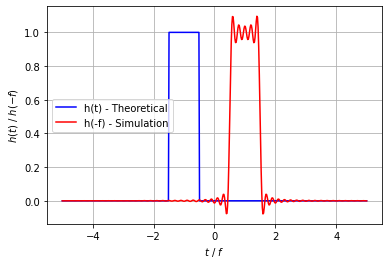
\includegraphics[width=\columnwidth]{signal_h_t.png}
    \caption{Plot of signals $h\brak{t}$ and $h\brak{-f}$}
    \label{fig:figure1}
\end{figure}
\begin{figure}[h]
    \centering
    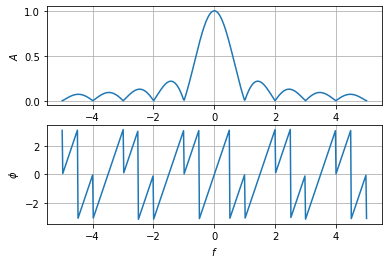
\includegraphics[width=\columnwidth]{signal_g_t.png}
    \caption{Plot of amplitude and phase of signal $g\brak{f}$}
    \label{fig:figure2}
\end{figure}
\end{document} 
